% Options for packages loaded elsewhere
\PassOptionsToPackage{unicode}{hyperref}
\PassOptionsToPackage{hyphens}{url}
\PassOptionsToPackage{dvipsnames,svgnames,x11names}{xcolor}
%
\documentclass[
  letterpaper,
  DIV=11,
  numbers=noendperiod]{scrreprt}

\usepackage{amsmath,amssymb}
\usepackage{iftex}
\ifPDFTeX
  \usepackage[T1]{fontenc}
  \usepackage[utf8]{inputenc}
  \usepackage{textcomp} % provide euro and other symbols
\else % if luatex or xetex
  \usepackage{unicode-math}
  \defaultfontfeatures{Scale=MatchLowercase}
  \defaultfontfeatures[\rmfamily]{Ligatures=TeX,Scale=1}
\fi
\usepackage{lmodern}
\ifPDFTeX\else  
    % xetex/luatex font selection
\fi
% Use upquote if available, for straight quotes in verbatim environments
\IfFileExists{upquote.sty}{\usepackage{upquote}}{}
\IfFileExists{microtype.sty}{% use microtype if available
  \usepackage[]{microtype}
  \UseMicrotypeSet[protrusion]{basicmath} % disable protrusion for tt fonts
}{}
\makeatletter
\@ifundefined{KOMAClassName}{% if non-KOMA class
  \IfFileExists{parskip.sty}{%
    \usepackage{parskip}
  }{% else
    \setlength{\parindent}{0pt}
    \setlength{\parskip}{6pt plus 2pt minus 1pt}}
}{% if KOMA class
  \KOMAoptions{parskip=half}}
\makeatother
\usepackage{xcolor}
\setlength{\emergencystretch}{3em} % prevent overfull lines
\setcounter{secnumdepth}{5}
% Make \paragraph and \subparagraph free-standing
\ifx\paragraph\undefined\else
  \let\oldparagraph\paragraph
  \renewcommand{\paragraph}[1]{\oldparagraph{#1}\mbox{}}
\fi
\ifx\subparagraph\undefined\else
  \let\oldsubparagraph\subparagraph
  \renewcommand{\subparagraph}[1]{\oldsubparagraph{#1}\mbox{}}
\fi

\usepackage{color}
\usepackage{fancyvrb}
\newcommand{\VerbBar}{|}
\newcommand{\VERB}{\Verb[commandchars=\\\{\}]}
\DefineVerbatimEnvironment{Highlighting}{Verbatim}{commandchars=\\\{\}}
% Add ',fontsize=\small' for more characters per line
\usepackage{framed}
\definecolor{shadecolor}{RGB}{241,243,245}
\newenvironment{Shaded}{\begin{snugshade}}{\end{snugshade}}
\newcommand{\AlertTok}[1]{\textcolor[rgb]{0.68,0.00,0.00}{#1}}
\newcommand{\AnnotationTok}[1]{\textcolor[rgb]{0.37,0.37,0.37}{#1}}
\newcommand{\AttributeTok}[1]{\textcolor[rgb]{0.40,0.45,0.13}{#1}}
\newcommand{\BaseNTok}[1]{\textcolor[rgb]{0.68,0.00,0.00}{#1}}
\newcommand{\BuiltInTok}[1]{\textcolor[rgb]{0.00,0.23,0.31}{#1}}
\newcommand{\CharTok}[1]{\textcolor[rgb]{0.13,0.47,0.30}{#1}}
\newcommand{\CommentTok}[1]{\textcolor[rgb]{0.37,0.37,0.37}{#1}}
\newcommand{\CommentVarTok}[1]{\textcolor[rgb]{0.37,0.37,0.37}{\textit{#1}}}
\newcommand{\ConstantTok}[1]{\textcolor[rgb]{0.56,0.35,0.01}{#1}}
\newcommand{\ControlFlowTok}[1]{\textcolor[rgb]{0.00,0.23,0.31}{#1}}
\newcommand{\DataTypeTok}[1]{\textcolor[rgb]{0.68,0.00,0.00}{#1}}
\newcommand{\DecValTok}[1]{\textcolor[rgb]{0.68,0.00,0.00}{#1}}
\newcommand{\DocumentationTok}[1]{\textcolor[rgb]{0.37,0.37,0.37}{\textit{#1}}}
\newcommand{\ErrorTok}[1]{\textcolor[rgb]{0.68,0.00,0.00}{#1}}
\newcommand{\ExtensionTok}[1]{\textcolor[rgb]{0.00,0.23,0.31}{#1}}
\newcommand{\FloatTok}[1]{\textcolor[rgb]{0.68,0.00,0.00}{#1}}
\newcommand{\FunctionTok}[1]{\textcolor[rgb]{0.28,0.35,0.67}{#1}}
\newcommand{\ImportTok}[1]{\textcolor[rgb]{0.00,0.46,0.62}{#1}}
\newcommand{\InformationTok}[1]{\textcolor[rgb]{0.37,0.37,0.37}{#1}}
\newcommand{\KeywordTok}[1]{\textcolor[rgb]{0.00,0.23,0.31}{#1}}
\newcommand{\NormalTok}[1]{\textcolor[rgb]{0.00,0.23,0.31}{#1}}
\newcommand{\OperatorTok}[1]{\textcolor[rgb]{0.37,0.37,0.37}{#1}}
\newcommand{\OtherTok}[1]{\textcolor[rgb]{0.00,0.23,0.31}{#1}}
\newcommand{\PreprocessorTok}[1]{\textcolor[rgb]{0.68,0.00,0.00}{#1}}
\newcommand{\RegionMarkerTok}[1]{\textcolor[rgb]{0.00,0.23,0.31}{#1}}
\newcommand{\SpecialCharTok}[1]{\textcolor[rgb]{0.37,0.37,0.37}{#1}}
\newcommand{\SpecialStringTok}[1]{\textcolor[rgb]{0.13,0.47,0.30}{#1}}
\newcommand{\StringTok}[1]{\textcolor[rgb]{0.13,0.47,0.30}{#1}}
\newcommand{\VariableTok}[1]{\textcolor[rgb]{0.07,0.07,0.07}{#1}}
\newcommand{\VerbatimStringTok}[1]{\textcolor[rgb]{0.13,0.47,0.30}{#1}}
\newcommand{\WarningTok}[1]{\textcolor[rgb]{0.37,0.37,0.37}{\textit{#1}}}

\providecommand{\tightlist}{%
  \setlength{\itemsep}{0pt}\setlength{\parskip}{0pt}}\usepackage{longtable,booktabs,array}
\usepackage{calc} % for calculating minipage widths
% Correct order of tables after \paragraph or \subparagraph
\usepackage{etoolbox}
\makeatletter
\patchcmd\longtable{\par}{\if@noskipsec\mbox{}\fi\par}{}{}
\makeatother
% Allow footnotes in longtable head/foot
\IfFileExists{footnotehyper.sty}{\usepackage{footnotehyper}}{\usepackage{footnote}}
\makesavenoteenv{longtable}
\usepackage{graphicx}
\makeatletter
\def\maxwidth{\ifdim\Gin@nat@width>\linewidth\linewidth\else\Gin@nat@width\fi}
\def\maxheight{\ifdim\Gin@nat@height>\textheight\textheight\else\Gin@nat@height\fi}
\makeatother
% Scale images if necessary, so that they will not overflow the page
% margins by default, and it is still possible to overwrite the defaults
% using explicit options in \includegraphics[width, height, ...]{}
\setkeys{Gin}{width=\maxwidth,height=\maxheight,keepaspectratio}
% Set default figure placement to htbp
\makeatletter
\def\fps@figure{htbp}
\makeatother

\KOMAoption{captions}{tableheading}
\makeatletter
\makeatother
\makeatletter
\@ifpackageloaded{bookmark}{}{\usepackage{bookmark}}
\makeatother
\makeatletter
\@ifpackageloaded{caption}{}{\usepackage{caption}}
\AtBeginDocument{%
\ifdefined\contentsname
  \renewcommand*\contentsname{Table of contents}
\else
  \newcommand\contentsname{Table of contents}
\fi
\ifdefined\listfigurename
  \renewcommand*\listfigurename{List of Figures}
\else
  \newcommand\listfigurename{List of Figures}
\fi
\ifdefined\listtablename
  \renewcommand*\listtablename{List of Tables}
\else
  \newcommand\listtablename{List of Tables}
\fi
\ifdefined\figurename
  \renewcommand*\figurename{Figure}
\else
  \newcommand\figurename{Figure}
\fi
\ifdefined\tablename
  \renewcommand*\tablename{Table}
\else
  \newcommand\tablename{Table}
\fi
}
\@ifpackageloaded{float}{}{\usepackage{float}}
\floatstyle{ruled}
\@ifundefined{c@chapter}{\newfloat{codelisting}{h}{lop}}{\newfloat{codelisting}{h}{lop}[chapter]}
\floatname{codelisting}{Listing}
\newcommand*\listoflistings{\listof{codelisting}{List of Listings}}
\makeatother
\makeatletter
\@ifpackageloaded{caption}{}{\usepackage{caption}}
\@ifpackageloaded{subcaption}{}{\usepackage{subcaption}}
\makeatother
\makeatletter
\@ifpackageloaded{tcolorbox}{}{\usepackage[skins,breakable]{tcolorbox}}
\makeatother
\makeatletter
\@ifundefined{shadecolor}{\definecolor{shadecolor}{rgb}{.97, .97, .97}}
\makeatother
\makeatletter
\makeatother
\makeatletter
\makeatother
\ifLuaTeX
  \usepackage{selnolig}  % disable illegal ligatures
\fi
\IfFileExists{bookmark.sty}{\usepackage{bookmark}}{\usepackage{hyperref}}
\IfFileExists{xurl.sty}{\usepackage{xurl}}{} % add URL line breaks if available
\urlstyle{same} % disable monospaced font for URLs
\hypersetup{
  pdftitle={Zelha Tunc Pekkan Progress Journal},
  colorlinks=true,
  linkcolor={blue},
  filecolor={Maroon},
  citecolor={Blue},
  urlcolor={Blue},
  pdfcreator={LaTeX via pandoc}}

\title{Zelha Tunc Pekkan Progress Journal}
\author{}
\date{}

\begin{document}
\maketitle
\ifdefined\Shaded\renewenvironment{Shaded}{\begin{tcolorbox}[frame hidden, boxrule=0pt, sharp corners, interior hidden, borderline west={3pt}{0pt}{shadecolor}, enhanced, breakable]}{\end{tcolorbox}}\fi

\renewcommand*\contentsname{Table of contents}
{
\hypersetup{linkcolor=}
\setcounter{tocdepth}{2}
\tableofcontents
}
\bookmarksetup{startatroot}

\hypertarget{introduction}{%
\chapter*{Introduction}\label{introduction}}
\addcontentsline{toc}{chapter}{Introduction}

\markboth{Introduction}{Introduction}

This progress journal covers Zelha Tunc Pekkan's work during their term
at \href{https://mef-bda503.github.io/fall23/}{BDA 503 Fall 2023}.

Each section is an assignment or an individual work.

\bookmarksetup{startatroot}

\hypertarget{assignment-1}{%
\chapter{Assignment 1}\label{assignment-1}}

I am a mathematics educator working with K-16 students and in-service
teachers. I am interested in how kids learn mathematics and how we can
teach them better. I hope that data science can help me to understand
how to model children's mathematical thinking and classroom interaction.
\href{https://www.linkedin.com/in/tuncpekkan/}{Here is my linkedin}

I watched the video ``How to Get Your Materials Online With R''
\href{\%22https://youtu.be/QcE4RBH2auQ?si=FfVFJoo9L9S9stqA}{Here is the
video}

Here is the summary: Educators create a lot of files for teaching-
slides, exercises, solutions, assignments, data, figures- that all
ultimately need to be shared with other people. Having a link for
sharing your teaching materials can save you time and pain, but it is
hard to get started if you've never shared your resources online before.
In this webinar, we'll give a tour of the R Markdown ecosystem for
educators that you can start to use right away. We'll show how it can
help you make your teaching more shareable, reproducible, and resilient.

The data set I propose is the PISA dataset. This is very challenging
\href{https://www.oecd.org/pisa/data/2015database/}{Here is the link}
but there are packages available such as:
\href{https://github.com/eldafani/intsvy}{Here is the link}

\href{https://www.r-bloggers.com/2016/12/pisa-2015-how-to-readprocessplot-the-data-with-r/}{Blog
1}
\href{https://www.r-bloggers.com/2015/06/analyze-the-trends-in-international-mathematics-and-science-study-timss-with-r/}{Blog
2}
\href{https://cran.r-project.org/web/packages/eeptools/vignettes/intro.html}{Blog
3}

PISA assesses the extent to which students near the end of compulsory
education have acquired some of the knowledge and skills that are
essential for full participation in society. It focuses on student
competencies in the key subject areas of reading, mathematics and
science.

\bookmarksetup{startatroot}

\hypertarget{inclass1-calculates-and-plots-pisa-data}{%
\chapter{inclass1: Calculates and Plots PISA
data}\label{inclass1-calculates-and-plots-pisa-data}}

\hypertarget{my-first-pisa-math-data-analysis}{%
\section{My first PISA Math data
analysis}\label{my-first-pisa-math-data-analysis}}

We used PISA 2015 data set
\url{https://www.oecd.org/pisa/data/2015database/}. This data set is too
big and there can easily be an entire class on this data set. The new
PISA data will be available on December 5, 2023! Check it out
\url{https://pisa2022-maths.oecd.org}

Original data is in SPSS format and a conversion function is used.

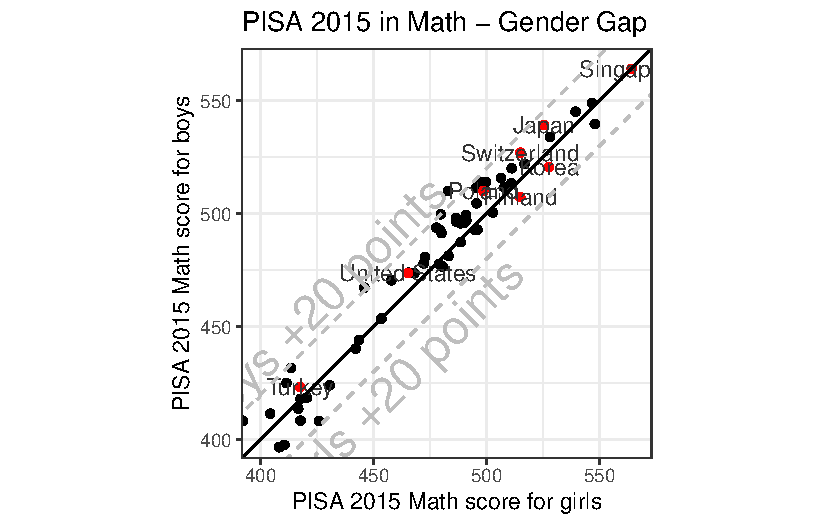
\includegraphics{inclass1_files/figure-pdf/plot-pisa-1.pdf}

\bookmarksetup{startatroot}

\hypertarget{inclass2.qmd}{%
\chapter{inclass2.qmd}\label{inclass2.qmd}}

\begin{Shaded}
\begin{Highlighting}[]
\FunctionTok{library}\NormalTok{(tidyverse)}
\end{Highlighting}
\end{Shaded}

\begin{verbatim}
-- Attaching core tidyverse packages ------------------------ tidyverse 2.0.0 --
v dplyr     1.1.3     v readr     2.1.4
v forcats   1.0.0     v stringr   1.5.0
v ggplot2   3.4.4     v tibble    3.2.1
v lubridate 1.9.3     v tidyr     1.3.0
v purrr     1.0.2     
-- Conflicts ------------------------------------------ tidyverse_conflicts() --
x dplyr::filter() masks stats::filter()
x dplyr::lag()    masks stats::lag()
i Use the conflicted package (<http://conflicted.r-lib.org/>) to force all conflicts to become errors
\end{verbatim}

\begin{Shaded}
\begin{Highlighting}[]
\FunctionTok{library}\NormalTok{(foreign)}

\FunctionTok{library}\NormalTok{(intsvy)}

\FunctionTok{library}\NormalTok{(dplyr)}

\FunctionTok{library}\NormalTok{(tidyr)}

\FunctionTok{library}\NormalTok{(ggplot2)}
\end{Highlighting}
\end{Shaded}

\begin{Shaded}
\begin{Highlighting}[]
\NormalTok{netflix}\OtherTok{=}\NormalTok{readr}\SpecialCharTok{::}\FunctionTok{read\_csv}\NormalTok{(}\StringTok{"netflix.csv"}\NormalTok{)}
\end{Highlighting}
\end{Shaded}

\begin{verbatim}
Rows: 1000 Columns: 7
-- Column specification --------------------------------------------------------
Delimiter: ","
chr (3): title, rating, ratinglevel
dbl (4): ratingdescription, release_year, user_rating_score, user_rating_size

i Use `spec()` to retrieve the full column specification for this data.
i Specify the column types or set `show_col_types = FALSE` to quiet this message.
\end{verbatim}

\begin{Shaded}
\begin{Highlighting}[]
\NormalTok{netflix}
\end{Highlighting}
\end{Shaded}

\begin{verbatim}
# A tibble: 1,000 x 7
   title     rating ratinglevel ratingdescription release_year user_rating_score
   <chr>     <chr>  <chr>                   <dbl>        <dbl>             <dbl>
 1 White Ch~ PG-13  crude and ~                80         2004                82
 2 Lucky Nu~ R      strong vio~               100         2006                NA
 3 Grey's A~ TV-14  Parents st~                90         2016                98
 4 Prison B~ TV-14  Parents st~                90         2008                98
 5 How I Me~ TV-PG  Parental g~                70         2014                94
 6 Supernat~ TV-14  Parents st~                90         2016                95
 7 Breaking~ TV-MA  For mature~               110         2013                97
 8 The Vamp~ TV-14  Parents st~                90         2017                91
 9 The Walk~ TV-MA  For mature~               110         2015                98
10 Pretty L~ TV-14  Parents st~                90         2016                96
# i 990 more rows
# i 1 more variable: user_rating_size <dbl>
\end{verbatim}

\begin{Shaded}
\begin{Highlighting}[]
\FunctionTok{ggplot}\NormalTok{(netflix }\SpecialCharTok{\%\textgreater{}\%} \FunctionTok{select}\NormalTok{(release\_year, user\_rating\_score) }\SpecialCharTok{\%\textgreater{}\%}
\FunctionTok{filter}\NormalTok{(}\FunctionTok{complete.cases}\NormalTok{(.)), }
\FunctionTok{aes}\NormalTok{(}\AttributeTok{x =}\NormalTok{ release\_year, }\AttributeTok{y =}\NormalTok{ user\_rating\_score)) }\SpecialCharTok{+} 
\FunctionTok{geom\_point}\NormalTok{()}\SpecialCharTok{+}
\FunctionTok{labs}\NormalTok{(}
  \AttributeTok{title=} \StringTok{"Movie Information"}\NormalTok{,}
  \AttributeTok{x=} \StringTok{"Year of the movie"}\NormalTok{,}
  \AttributeTok{y=} \StringTok{"User Rating"}
\NormalTok{  )}
\end{Highlighting}
\end{Shaded}

\begin{figure}[H]

{\centering 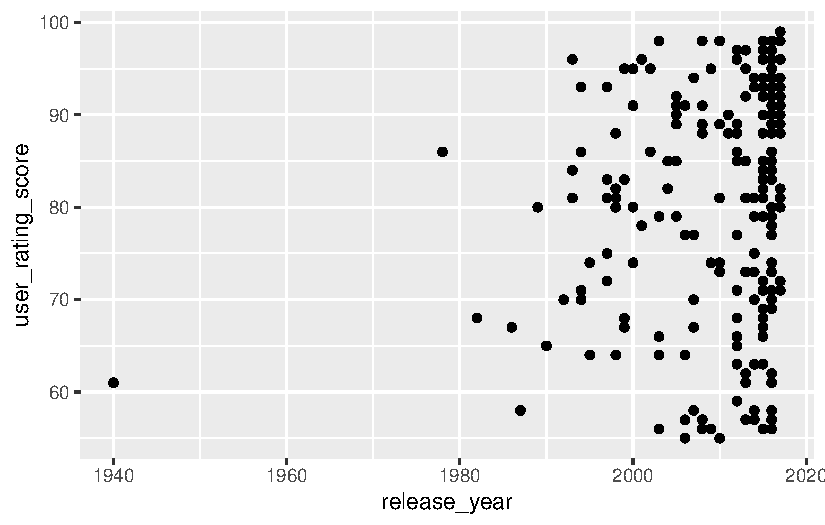
\includegraphics{inclass2_files/figure-pdf/unnamed-chunk-3-1.pdf}

}

\end{figure}

\bookmarksetup{startatroot}

\hypertarget{shiny}{%
\chapter{SHINY}\label{shiny}}

SHINY

Here is my Shiny Project:

Here you can select 3 countries, and three levels of performance in 2022
PISA math test (level 1 (low), Level 3, (medium) and Level 6 (high)
performing students Percentage.) You can also choose whether it is
\textbf{Government (g)} or \textbf{Private(p)} schools and within those
schools how they perform: for example, \% of government schools that
perform on low level will be \textbf{\emph{glevel1a}}

\url{https://foxy.shinyapps.io/try_shine/}

\bookmarksetup{startatroot}

\hypertarget{or-assignment}{%
\chapter{OR Assignment}\label{or-assignment}}

\#\#\textbf{OR Assignment - Examine a Case (Deadline: Jan 4, 23:59)}

In this individual assignment you are asked to choose a real life case
study solved with Operations Research and briefly describe it with your
own words.

\begin{itemize}
\item ~
  \hypertarget{problem-what-courses-to-take-from-online-platforms-for-data-science-so-we-can-finish-the-program-requirements-and-pay-just-enough}{%
  \section{Problem: What courses to take from online platforms for Data
  science so we can finish the program requirements and pay just
  enough?}\label{problem-what-courses-to-take-from-online-platforms-for-data-science-so-we-can-finish-the-program-requirements-and-pay-just-enough}}

  A student has 8 semesters to complete an online program, Total time T.

  Takes 3 courses per semester = 24 courses.

  \hypertarget{solution-decision-variables}{%
  \section{Solution: Decision
  Variables}\label{solution-decision-variables}}

  Ci is the total cost of course i.

  1) Min Total Cost of Courses = Sigma (i) (Ci).~ (Objective function to
  minimize total spending)

  2) Does the set of constrains to satisfy the required curriculum
  objectives (course contents)

  Ai,j: Contents of course i, for content j

  bj: Required corse content of content j.
\item
  Solution and Model:
\end{itemize}

Similar to the Model for the solution of the Diet problem
(or~\href{https://en.wikipedia.org/wiki/Stigler_diet}{Stigler Diet})



\end{document}
